%%%%%%%%%%%%%%%%%%%%%%%%%%%%%%%%%%%%%%%%%%%%%%%%%%%%%%%%%%%%
%%  This Beamer template was created by Cameron Bracken.
%%  Anyone can freely use or modify it for any purpose
%%  without attribution.
%%
%%  Last Modified: January 9, 2009
%%

\documentclass[xcolor=x11names,compress]{beamer}

%% General document %%%%%%%%%%%%%%%%%%%%%%%%%%%%%%%%%%
\usepackage{listings}
\usepackage{epstopdf}
\usepackage{graphicx}
\usepackage{tikz}
\usepackage[french]{babel}
\usepackage[T1]{fontenc}
\usepackage[utf8]{inputenc}
\usepackage{array}
\usepackage{svg}
\usepackage{calc}
\usetikzlibrary{decorations.fractals, calc}
%%%%%%%%%%%%%%%%%%%%%%%%%%%%%%%%%%%%%%%%%%%%%%%%%%%%%%

\definecolor{bg-color}{HTML}{F26E27}
\definecolor{green-avantages}{HTML}{23B854}
\newcommand{\firstlogo}{images/m2dl.png}
\newcommand{\secondlogo}{images/ups.jpg}
\newcommand{\footsubject}{Git, essayons de reprendre le contrôle !} % Subject in footer

%% Beamer Layout %%%%%%%%%%%%%%%%%%%%%%%%%%%%%%%%%%
\mode<presentation> {
	\usepackage{../../../LaTeX-Beamer-Theme/beamerthemeShortPresentation}
}
%%%%%%%%%%%%%%%%%%%%%%%%%%%%%%%%%%%%%%%%%%%%%%%%%%

\setbeamercovered{invisible}

\AtBeginSection[]{%
  \begin{frame}<beamer>
  \tableofcontents[currentsection]
  \end{frame}
}

\definecolor{gris1}{gray}{0.40}
\definecolor{gris2}{gray}{0.55}
\definecolor{gris3}{gray}{0.65}
\definecolor{gris4}{gray}{0.50}
\definecolor{vert}{rgb}{0,0.4,0}
\definecolor{violet}{rgb}{0.65, 0.2, 0.65}
\definecolor{bleu1}{rgb}{0,0,0.8}
\definecolor{bleu2}{rgb}{0,0.2,0.6}
\definecolor{bleu3}{rgb}{0,0.2,0.2}
\definecolor{rouge}{HTML}{F93928}


\lstdefinelanguage{algo}{%
   morekeywords={%
    %%% couleur 1
		importer, programme, glossaire, Procedure, is, fonction, procedure, constante, type, 
	%%% IMPORT & Co.
		si, sinon, while, endloop, switch, alors, fin, tantque, debut, faire, lorsque, fin lorsque, 
		declenche, declencher, enregistrement, tableau, retourne, retourner, =, pour, a,
		/=, <, >, traite,exception, 
	%%% types 
		Entier, Reel, Booleen, Caractere, Réél, Booléen, Caractère,
	%%% types 
		entree, maj, sortie,entrée,
	%%% types 
		et, ou, non,
		Debut, début, debut, fin, Fin, faux, vrai, Faux, Vrai
	},
  sensitive=false,
  morecomment=[l]{--},
  morecomment=[l]{//},
  morestring=[b]',
}

\lstset{language=algo,
    %%% BOUCLE, TEST & Co.
      emph={importer, programme, glossaire, Procedure, is, fonction, procedure, constante, type},
      emphstyle=\color{bleu2},
    %%% IMPORT & Co.  
	emph={[2]
		si, sinon, while, endloop, switch, alors, fin , tantque, debut, faire, lorsque, fin lorsque, 
		declencher, retourner, et, ou, non,enregistrement, retourner, retourne, 
		tableau, /=, <, =, >, traite,exception, pour, a
	},
      emphstyle=[2]\color{bleu1},
    %%% FONCTIONS NUMERIQUES
		emph={[3]Vrai, vrai, Faux, faux},
      emphstyle=[3]\color{red},
    %%% FONCTIONS NUMERIQUES
      emph={[4]entree, maj, sortie, entrée},	
      emphstyle=[4]\color{gris1},
}
\lstdefinelanguage{wl}{%
   morekeywords={%
    %%% couleur 1
		importer, programme, glossaire, fonction, procedure, constante, type, 
	%%% IMPORT & Co.
		si, sinon, alors, fin, TANTQUE, tantque, FIN, PROCEDURE, debut, faire, lorsque, 
		fin lorsque, declenche, declencher, enregistrement, tableau, retourne, retourner, =, 
		/=, <, >, traite,exception, 
	%%% types 
		Entier, Reel, Booleen, Caractere, Réél, Booléen, Caractère,
	%%% types 
		entree, maj, sortie,entrée,
	%%% types 
		et, ou, non,
	},
  sensitive=true,
  morecomment=[l]{//},
  morestring=[b]',
}

\lstset{language=wl,
    %%% BOUCLE, TEST & Co.
      emph={importer, programme, glossaire, fonction, procedure, constante, type},
      emphstyle=\color{bleu2},
    %%% IMPORT & Co.  
	emph={[2]
		si, sinon, alors, fin , tantque, debut, faire, lorsque, fin lorsque, 
		declencher, retourner, et, ou, non,enregistrement, retourner, retourne, 
		tableau, /=, <, =, >, traite,exception
	},
      emphstyle=[2]\color{bleu1},
    %%% FONCTIONS NUMERIQUES
%      emph={[3]Entier, Reel, Booleen, Caractere, Booléen, Réél, Caractère},
 %     emphstyle=[3]\color{gris1},
    %%% FONCTIONS NUMERIQUES
      emph={[4]entree, maj, sortie, entrée},	
      emphstyle=[4]\color{gris1},
}
\lstdefinelanguage{css}{%
   morekeywords={%
    %%% couleur 1
		background, image, repeat, position, index, color, border, font, 
		size, url, family, style, variant, weight, letter, spacing, line, 
		height, text, decoration, align, indent, transform, shadow, 
		background, image, repeat, position, index, color, border, font, 
		size, url, family, style, variant, weight, letter, spacing, line, 
		height, text, decoration, align, indent, transform, shadow, 
		vertical, align, white, space, word, spacing,attachment, width, 
		max, min, margin, padding, clip, direction, display, overflow,
		visibility, clear, float, top, right, bottom, left, list, type, 
		collapse, side, empty, cells, table, layout, cursor, marks, page, break,
		before, after, inside, orphans, windows, azimuth, after, before, cue, 
		elevation, pause, play, during, pitch, range, richness, spek, header, 
		numeral, punctuation, rate, stress, voice, volume,
	%%% types 
		left, right, bottom, top, none, center, solid, black, blue, red, green,
	},
  sensitive=true,
  sensitive=true,
  morecomment=[s]{/*}{*/},
  morestring=[b]',
}
\lstset{language=css,
    %%% BOUCLE, TEST & Co.
      emph={
		background, image, repeat, position, index, color, border, font, 
		size, url, family, style, variant, weight, letter, spacing, line, 
		height, text, decoration, align, indent, transform, shadow, 
		background, image, repeat, position, index, color, border, font, 
		size, url, family, style, variant, weight, letter, spacing, line, 
		height, text, decoration, align, indent, transform, shadow, 
		vertical, align, white, space, word, spacing,attachment, width, 
		max, min, margin, padding, clip, direction, display, overflow,
		visibility, clear, float, top, right, bottom, left, list, type, 
		collapse, side, empty, cells, table, layout, cursor, marks, page, break,
		before, after, inside, orphans, windows, azimuth, after, before, cue, 
		elevation, pause, play, during, pitch, range, richness, spek, header, 
		numeral, punctuation, rate, stress, voice, volume,
	  },
      emphstyle=\color{bleu2},
    %%% FONCTIONS NUMERIQUES
      emph={[3]
		left, right, bottom, top,none, solid, black, blue, green,
		  },
      emphstyle=[3]\color{bleu3},
    %%% FONCTIONS NUMERIQUES
}

\lstset{language=SQL,
    %%% BOUCLE, TEST & Co.
      emph={INSERT, UPDATE, DELETE, WHERE, SET, GROUP, BY, ORDER, REFERENCES},
      emphstyle=\color{bleu2},
    %%% IMPORT & Co.  
	emph={[2]
		if, end, begin, then, for, each, else, after, of, on, to
	},
      emphstyle=[2]\color{bleu1},
    %%% FONCTIONS NUMERIQUES
%      emph={[3]Entier, Reel, Booleen, Caractere, Booléen, Réél, Caractère},
 %     emphstyle=[3]\color{gris1},
    %%% FONCTIONS NUMERIQUES
      emph={[4]entree, maj, sortie, entrée},	
      emphstyle=[4]\color{gris1},
}
\lstdefinelanguage{ARM}{%
   morekeywords={%
   ADD, SUB, MOV, MUL, RSB,CMP, BLS, BLE, B,BHI,LDR,
   BGE, RSBLT, BGT, BEQ, BNE,BLT,BHS,STR,STRB,ADR, LDMFD, STMFD, LDRB
	},
  sensitive=true,
  morecomment=[l]{@},
  morestring=[b]',
}

\lstdefinelanguage{javascript}{
   morekeywords={%
		if, while, else
	},
  sensitive=true,
  comment=[s]{/*}{*/},
  morecomment=[l]{//},
  string=[b]',
  morestring=[b]",
}
\lstdefinelanguage{PHP}{
   morekeywords={%
	foreach, echo, include, div, a, as, return, while, function, array
	},
  sensitive=true,
  morecomment=[s]{<!--}{-->},
  morecomment=[s]{/*}{*/},
  morecomment=[l]{//},
  string=[b]',
  morestring=[b]",
}
\lstset{language=Caml,
    %%% BOUCLE, TEST & Co.
      emph={int,bool, float},
      emphstyle=\color{bleu2},
}

\lstset{ % general style for listings 
   numbers=left 
   , literate={é}{{\'e}}1 {è}{{\`e}}1 {à}{{\`a}}1 {ê}{{\^e}}1 {É}{{\'E}}1 {ô}{{\^o}}1 {€}{{\euro}}1{°}{{$^{\circ}$}}1 {ç}{ {c}}1 {ù}{u}1
	, extendedchars=\true
   , tabsize=2 
   , stepnumber=2
   , frame=l
   , framerule=1.1pt
   , linewidth=510px
   , breaklines=true 
   , basicstyle=\footnotesize\ttfamily 
   , numberstyle=\tiny\ttfamily 
   , framexleftmargin=0mm 
   , xleftmargin=0mm 
   , captionpos=b 
	, keywordstyle=\color{bleu2}
	, commentstyle=\color{vert}
	, stringstyle=\color{rouge}
	, showstringspaces=false
	, extendedchars=true
	, mathescape=true
	, prebreak=\raisebox{0ex}[0ex][0ex]
		   {\ensuremath{\hookleftarrow}}
	,breakatwhitespace=true
} 
%	\lstlistoflistings
%	\addcontentsline{toc}{part}{List of code examples}


\begin{document}


%%%%%%%%%%%%%%%%%%%%%%%%%%%%%%%%%%%%%%%%%%%%%%%%%%%%%%
%%%%%%%%%%%%%%%%%%%%%%%%%%%%%%%%%%%%%%%%%%%%%%%%%%%%%%
\begin{frame}
\title{\centering Git, Essayons de reprendre le contrôle !}
\subtitle{}
\author{
	\centering
  Antoine de {\sc Roquemaurel}\\
	  \begin{tabular}{ccc}
		  
\includegraphics[height=7pt]{images/twitter.png}~satenske
	  \end{tabular}
	  \\
  {\footnotesize
	  \vspace{10px}
		Développeur Java consultant chez Tech Advantage\\
  }
}
\date{
	{
	  \begin{tabular}{ccc}
		  
\includegraphics[height=1.cm]{images/logo_extia}\hspace{20px} & 
		  
\includegraphics[height=1.cm]{images/meetup_by_extia} & 
		  \hspace{10px} 
\includegraphics[height=1cm]{images/logo_git}
	  \end{tabular}
	}
	\\
	\vspace{10px}
	Meetup Java / C\# du 28 Mars 2019\\\vspace{0.9cm}
	\vfill
	\includegraphics[width=1cm]{images/cc-by.eps} 
	\begin{minipage}{0.8\textwidth} 
		\tiny Cette œuvre est mise à disposition selon les termes de la Licence Creative Commons By 4.0\\
	\end{minipage}
}
\titlepage
\end{frame}

\begin{frame}{Le logiciel de gestion de versions}
	\begin{figure}[H]
		\includegraphics[width=9.4cm]{images/intro/cvs.png}
		\vspace{-10px}
		\caption{Pourquoi devrais-je utiliser le contrôle de version ?\footnote{\tiny\url{https://stackoverflow.com/questions/1408450/why-should-i-use-version-control}}}
	\end{figure}
\end{frame}

\begin{frame}{Git}
	\vspace{-1cm}
	\begin{tabular}{ll}
		\begin{minipage}{4.0cm}
		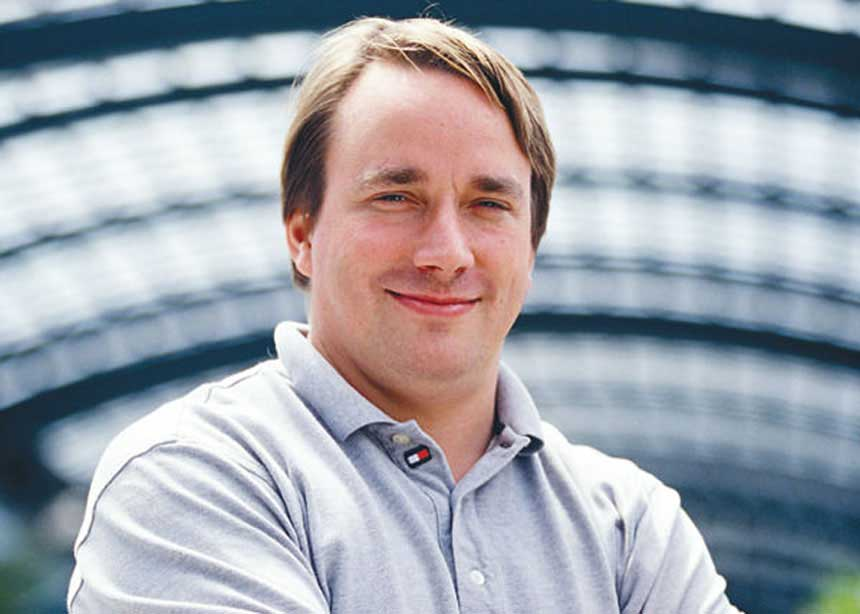
\includegraphics[width=4cm]{images/linus.jpg} 
		\end{minipage}
		&
		\begin{minipage}{0.6\textwidth}
		\vspace{60px}
			\begin{itemize}
				\item<1-> Créé en 2005 par {Linus Torvalds}
				\item<1-> Décentralisé
				\item<1-> Excellente gestion des branches
				\item<1-> Efficace sur de gros projet
					\uncover<2> {
					\begin{itemize}
						\item Microsoft Windows : 
					\tiny{
					\begin{itemize}
						\item 3 500 000 fichiers, soit 300 Go
						\item 440 branches
						\item 4 000 utilisateurs 
						\item 10 000 merges 
					\end{itemize}
					}
					\end{itemize}
					}
			\end{itemize}
		\end{minipage}
	\end{tabular}

	\uncover<3>{
		\vfill
		\centering
		<< \textit{I'm an egotistical bastard, and I name all my projects after myself. First 'Linux', now 'git'.} >>
		\vspace{30px}
	}
\end{frame}

\section{Fonctionnement de Git}
\begin{frame}{Le système décentralisé}
	\begin{figure}[H]
		\centering
		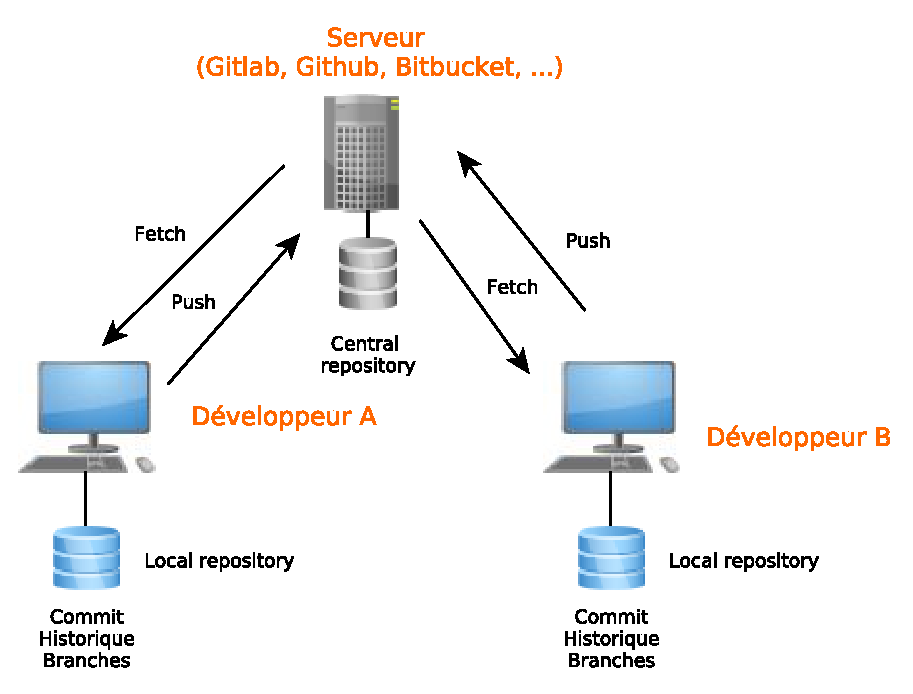
\includegraphics[width=8.5cm]{images/1-bases/git-repo.eps}
		\caption{Système décentralisé}
	\end{figure}
\end{frame}

\begin{frame}{La zone de transit (\textit{staging area})}
	\begin{figure}[H]
		\vspace{-10px}
		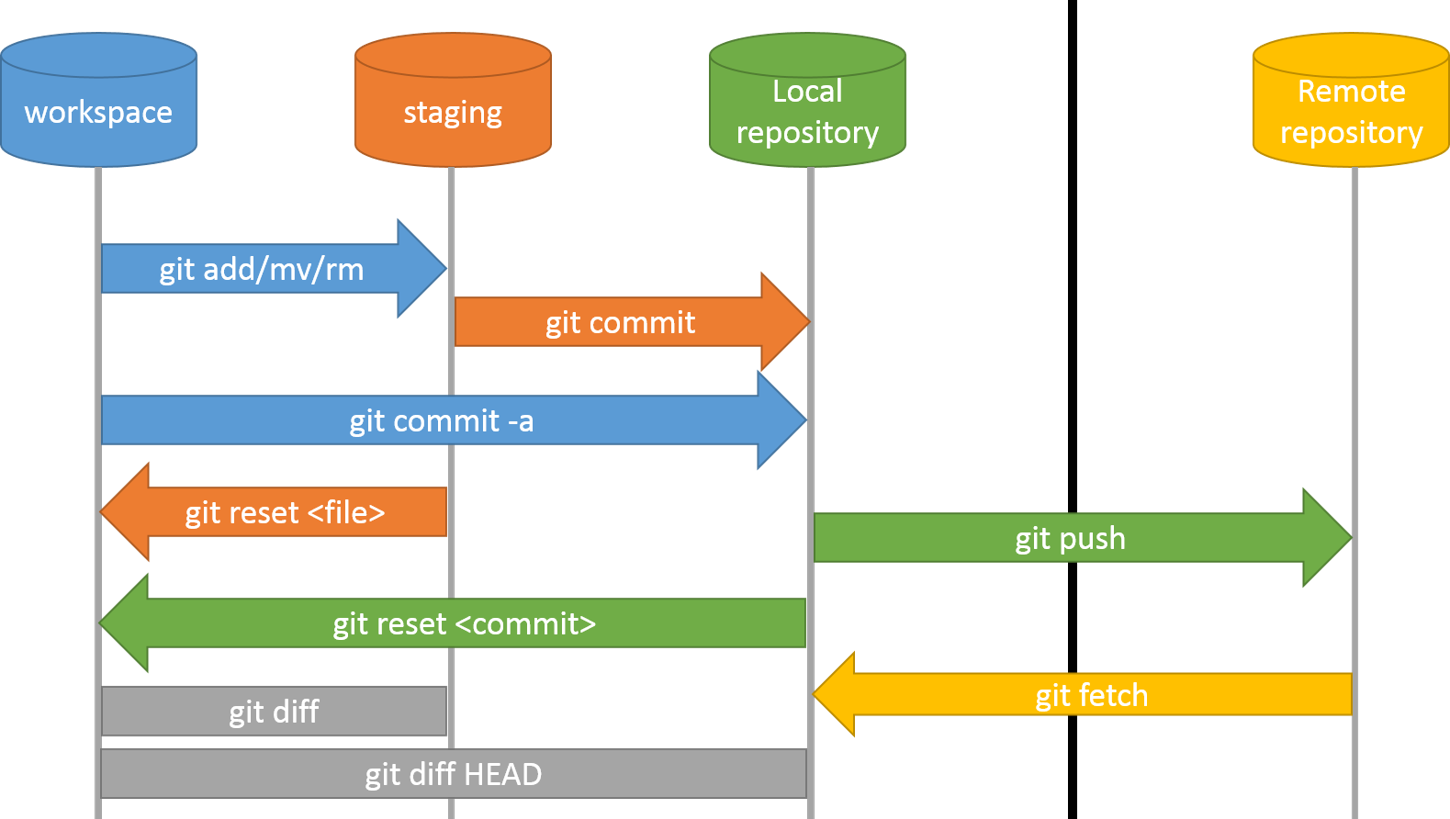
\includegraphics[width=11cm]{images/1-bases/staging.png}
		\caption{Fonctionnement de Git}
	\end{figure}	
\end{frame}

\section{Dans les coulisses}
\begin{frame}{Le stockage des données du dépôt : les objets}
		\begin{itemize}
			\item<1-> Les changements de fichiers sont stockés dans le \textbf{commit}
			\item<2-> Un \textbf{tree} représente un niveau de hiérarchie de fichiers
			\item<3-> Chaque version de chaque fichier est un \textbf{blob}
			\item<4-> Les \textbf{commits} sont chainés entre eux
			\item<5-> Les \textbf{tags}, \textbf{branches} et \textbf{HEAD} sont des pointeurs de commit
		\end{itemize}
		\begin{figure}[H]
			\centering
			\only<1>{
			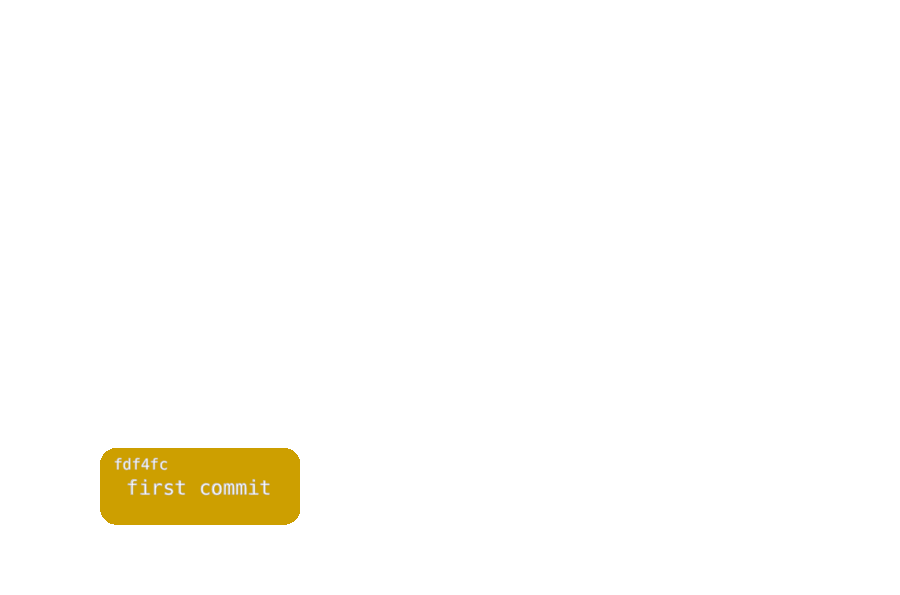
\includegraphics[width=7cm]{images/2-coulisses/data-model-1.png}
			}
			\only<2>{
			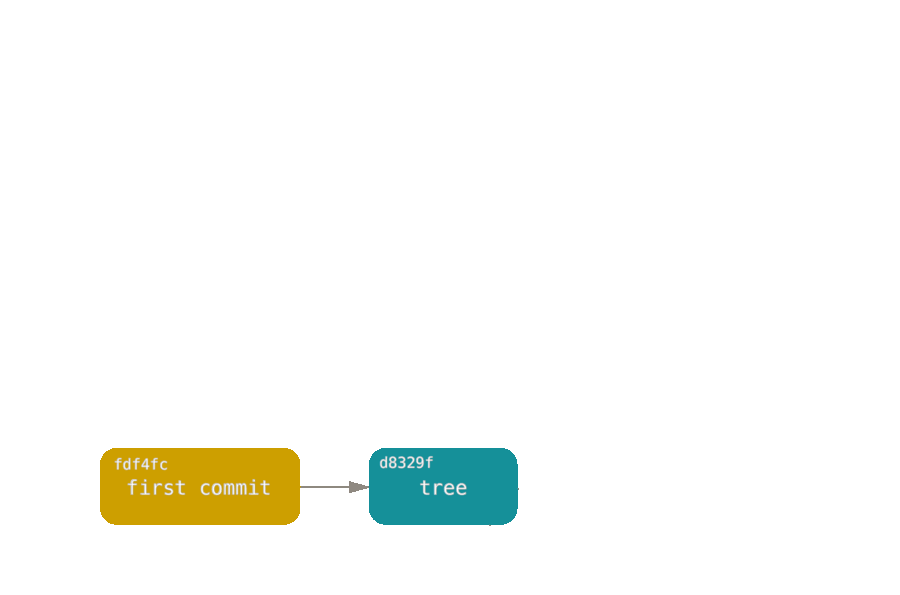
\includegraphics[width=7cm]{images/2-coulisses/data-model-2.png}
			}
			\only<3>{
			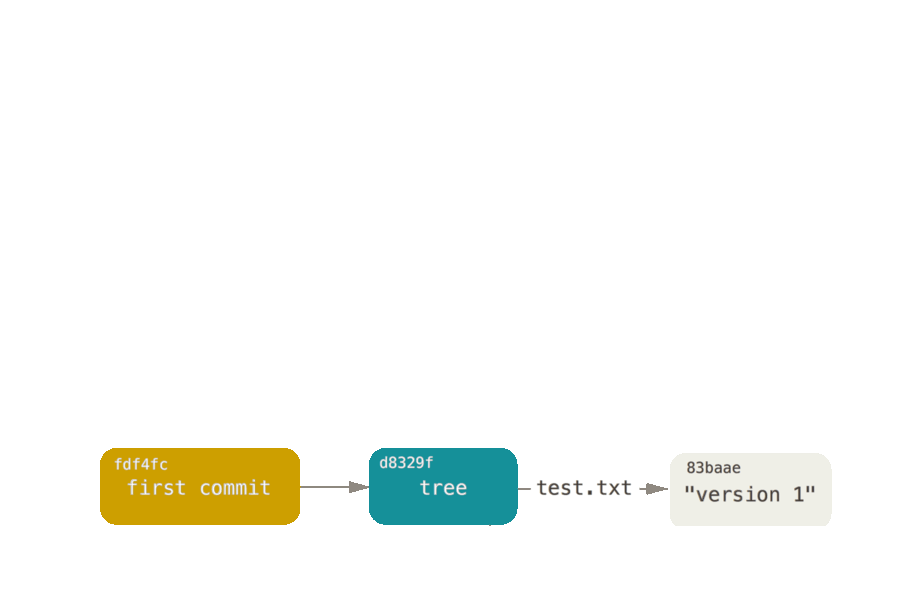
\includegraphics[width=7cm]{images/2-coulisses/data-model-3.png}
			}
			\only<4>{
			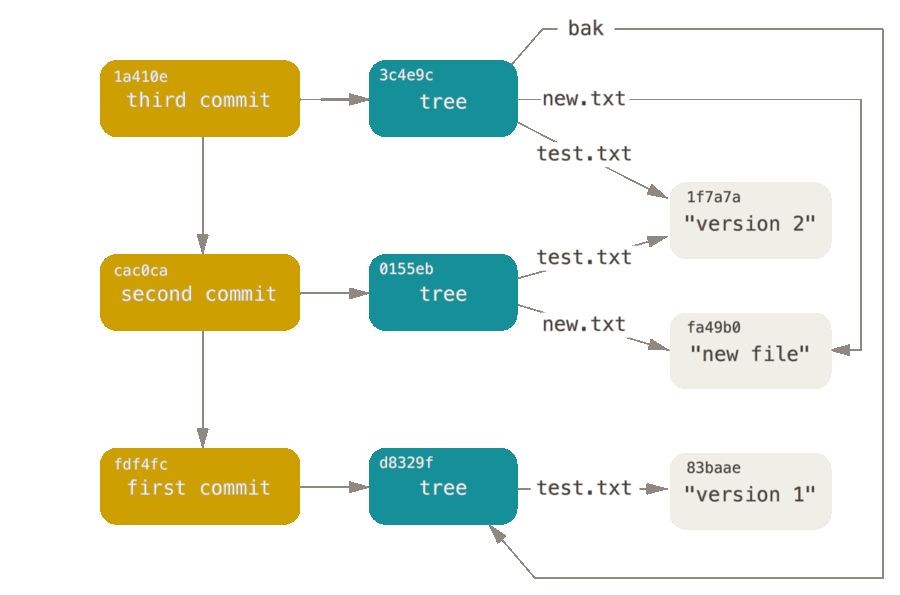
\includegraphics[width=7cm]{images/2-coulisses/data-model-4.png}
			}
			\only<5>{
			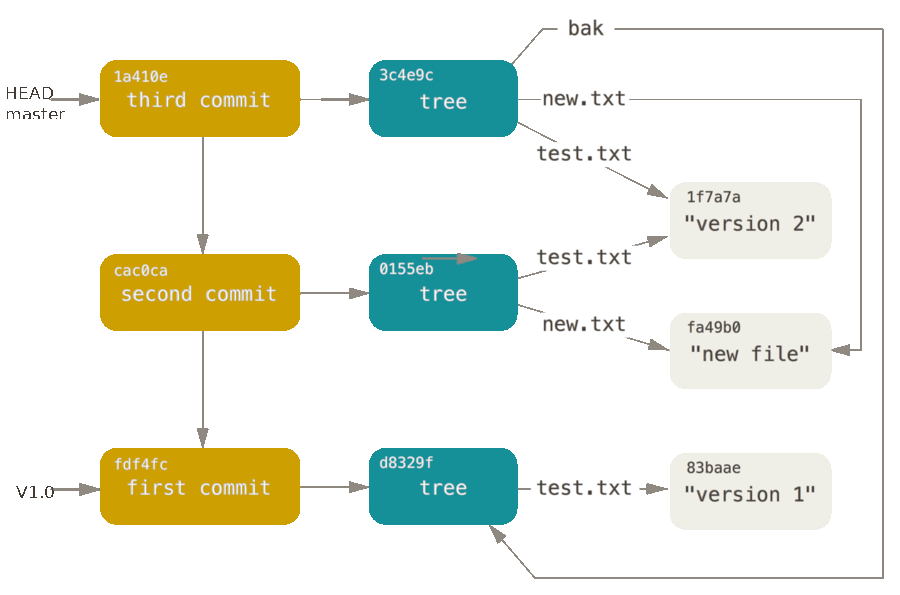
\includegraphics[width=7cm]{images/2-coulisses/data-model.png}
			}
		\end{figure}
\end{frame}
\begin{frame}{Le stockage des infos du workspace : l'index}
	\begin{itemize}
		\item Le fichier contient toutes les informations nécessaires à la génération d'un \textit{tree object}
			\vfill
		\item Il permet la comparaison rapide entre un \textit{tree object} et le \textit{working tree}
			\vfill
		\item Il contient les informations sur les \textit{merges conflicts}
	\end{itemize}
\end{frame}

\begin{frame}{Git débite à la hash !}
	\begin{itemize}
		\item Tout objet du store est adressable par son contenu
			\vfill
		\item Le nom unique de chaque objet est obtenu avec \texttt{SHA-1}\\
			\begin{itemize}
				\item Valeur sur 160 bits (nombre hexadécimal à 40 chiffres)
			\end{itemize}
			\vfill
		\item Toute modification du contenu produira un changement du hash
	\end{itemize}
\end{frame}

%\begin{frame}{Les actions de base}
%\begin{itemize}
%	\item \texttt{commit}
%	\item \texttt{fetch}
%	\item \texttt{push}
%	\item \texttt{blame}
%\end{itemize}
%\end{frame}
% Git débite à la hash

\section{La collaboration}
\begin{frame}{Restons branchés : le Git-flow}
	\begin{figure}[H]
		\centering
		\only<1>{
		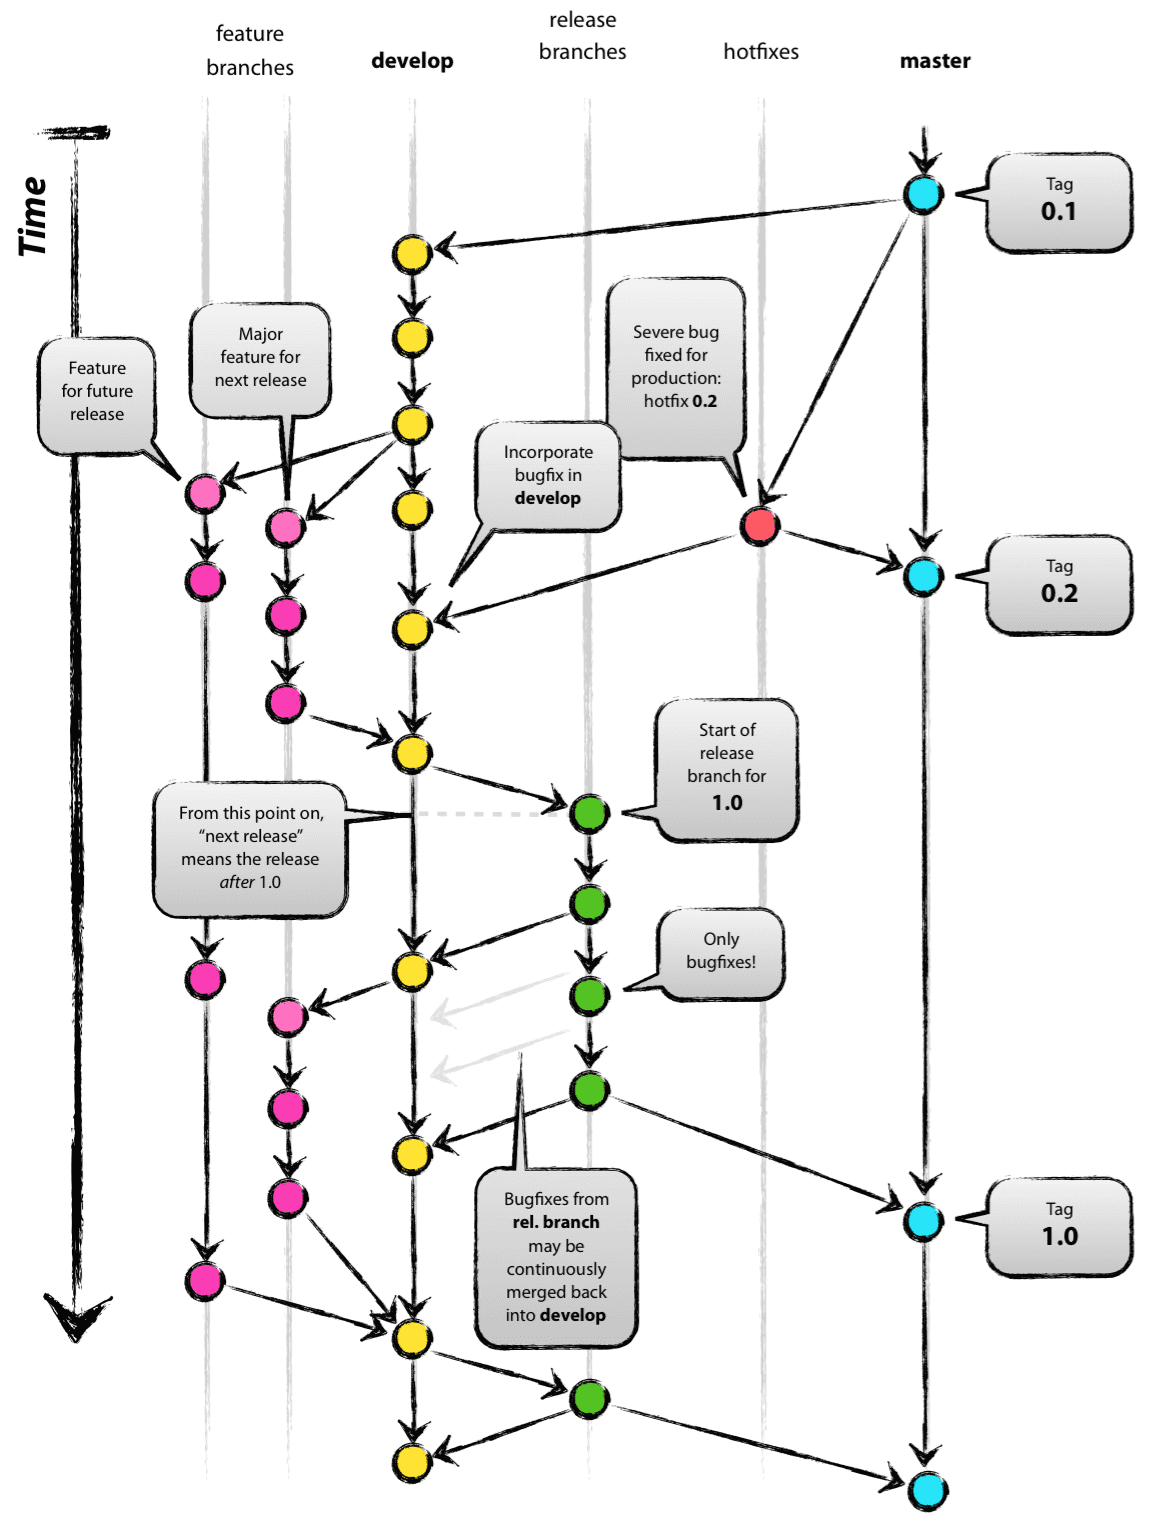
\includegraphics[height=0.7\textheight]{images/2-workflow/gitflow.png}
		\caption{Un modèle de branchement\footnote{\tiny \url{https://nvie.com/posts/a-successful-git-branching-model/}}}
		}
		\only<2>{
		\vspace{-1.5cm}
		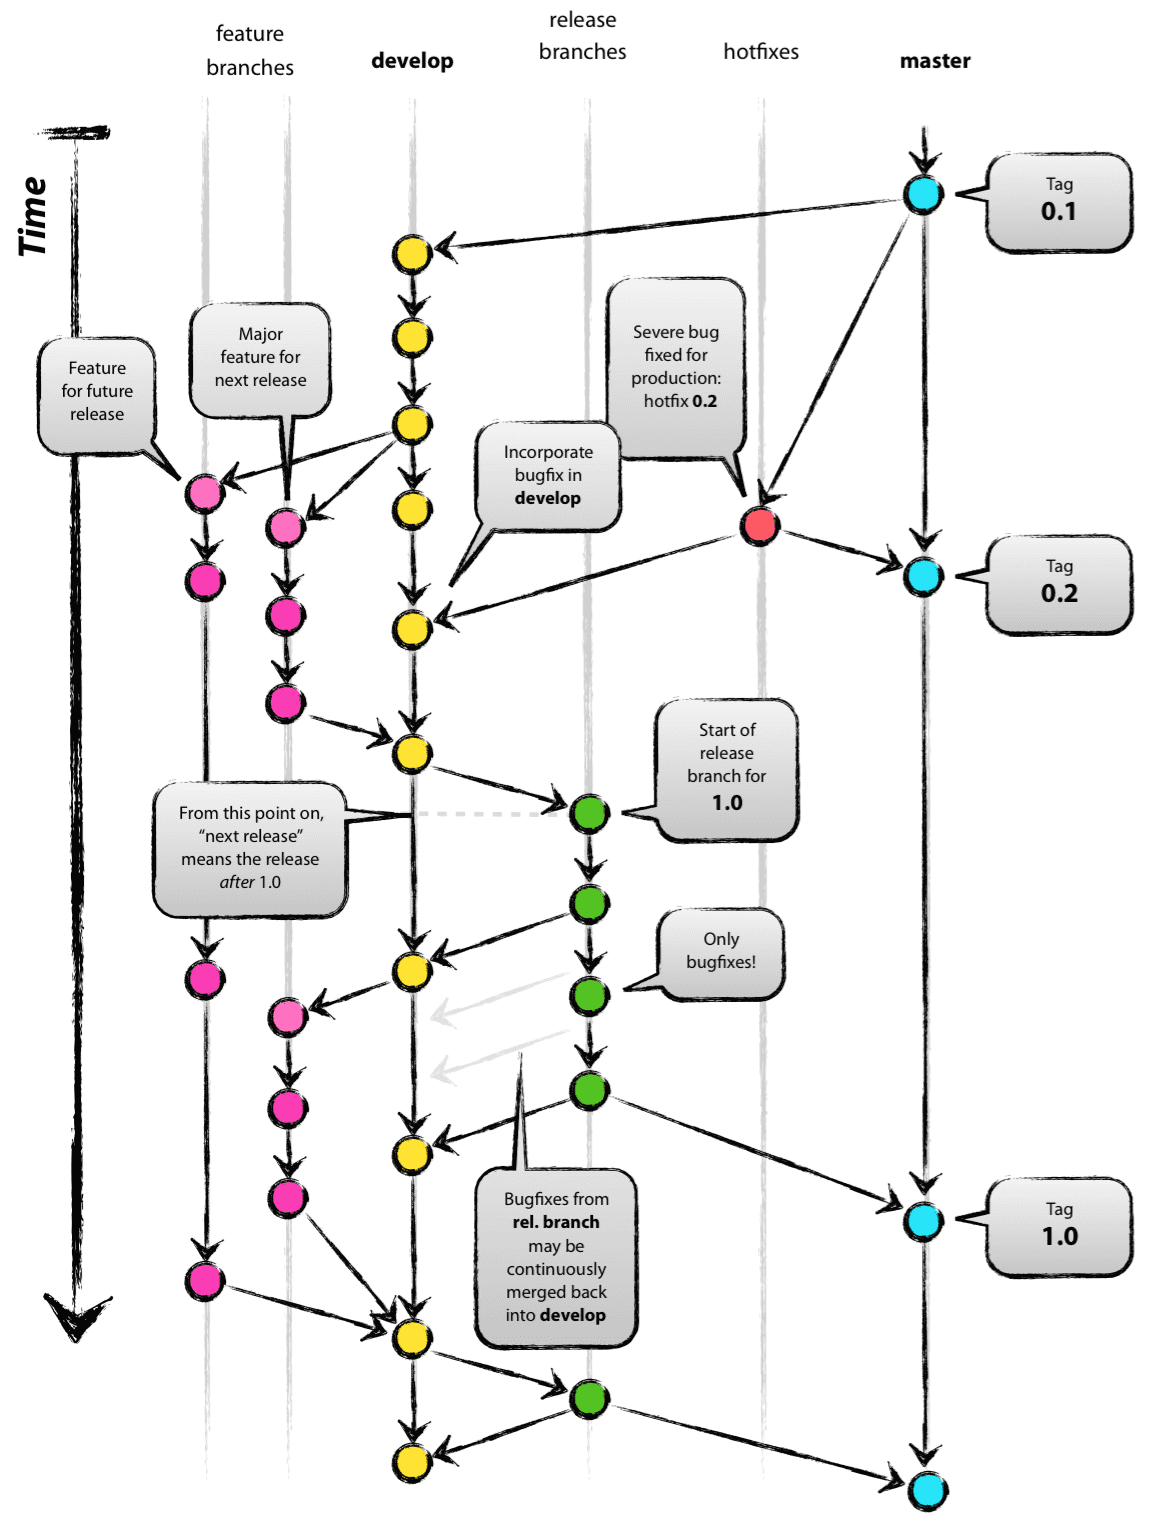
\includegraphics[height=1.1\textheight]{images/2-workflow/gitflow.png}
		}
	\end{figure}
\end{frame}

\begin{frame}{De l'importance de l'historique}
	\begin{tabular}{lc}
	\begin{minipage}{0.4\textwidth}
	Ingrédients : 
	\begin{itemize}
		\item 200g de beurre
		\item 200g de chocolat
		\item 4 œufs
		\item 150g de sucre
		\item 60g de farine
		\item $\frac{1}{2}$ sachet de levure
	\end{itemize}
	\end{minipage}
	&
	\begin{minipage}{0.6\textwidth}
		\begin{figure}[H]
			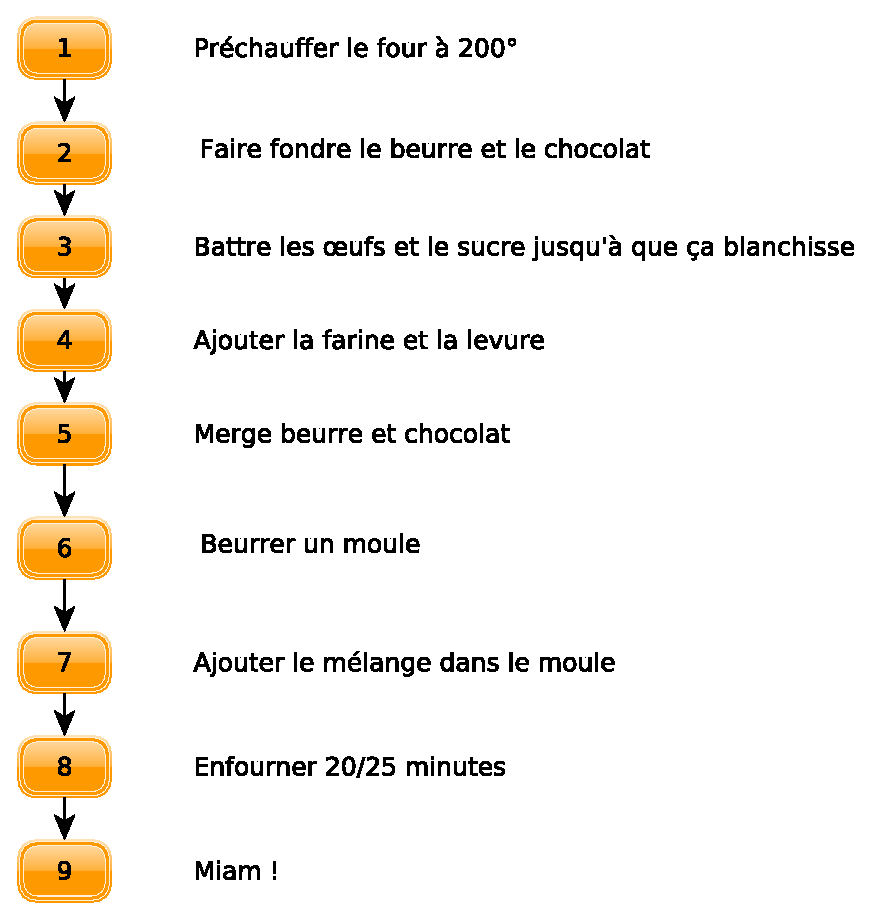
\includegraphics[width=5.5cm]{images/3-collaboration/sansbranche.eps}
			\caption{Historique sans collaboration}
		\end{figure}
	\end{minipage}
	\end{tabular}

\end{frame}
\begin{frame}{Le merge : on parralélise}
	\begin{figure}[H]
		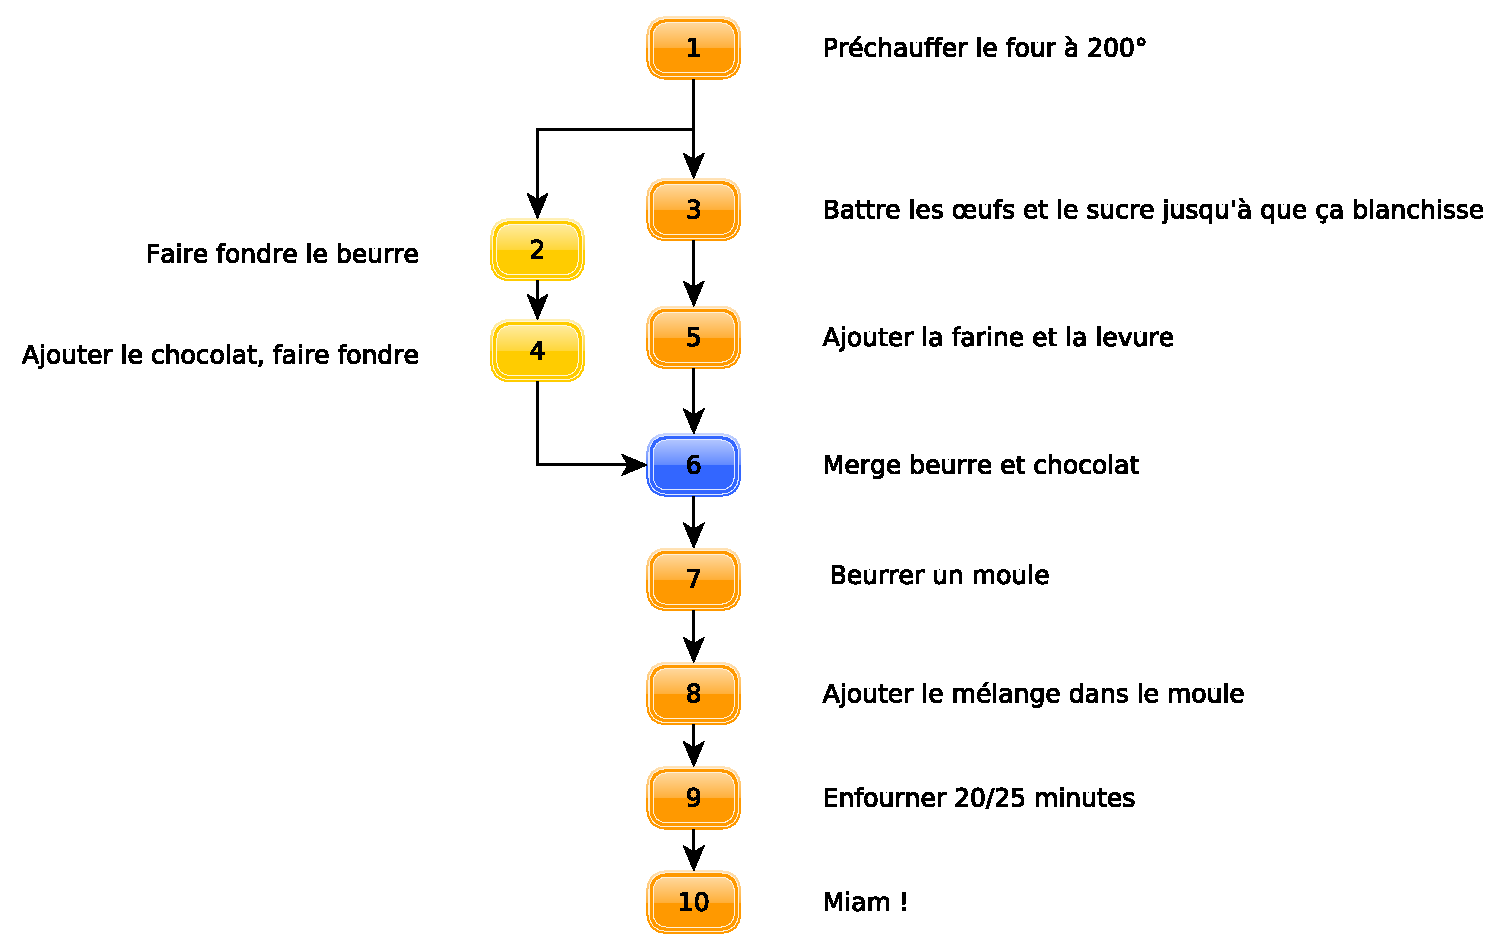
\includegraphics[width=9cm]{images/3-collaboration/merge.eps}
	\end{figure}
	\lstinputlisting[language=sh]{merge}%
\end{frame}
\begin{frame}{Le merge : le fast-forward}
	\begin{tabular}{cc}
		\begin{minipage}{0.5\textwidth}
			\uncover<1->{
				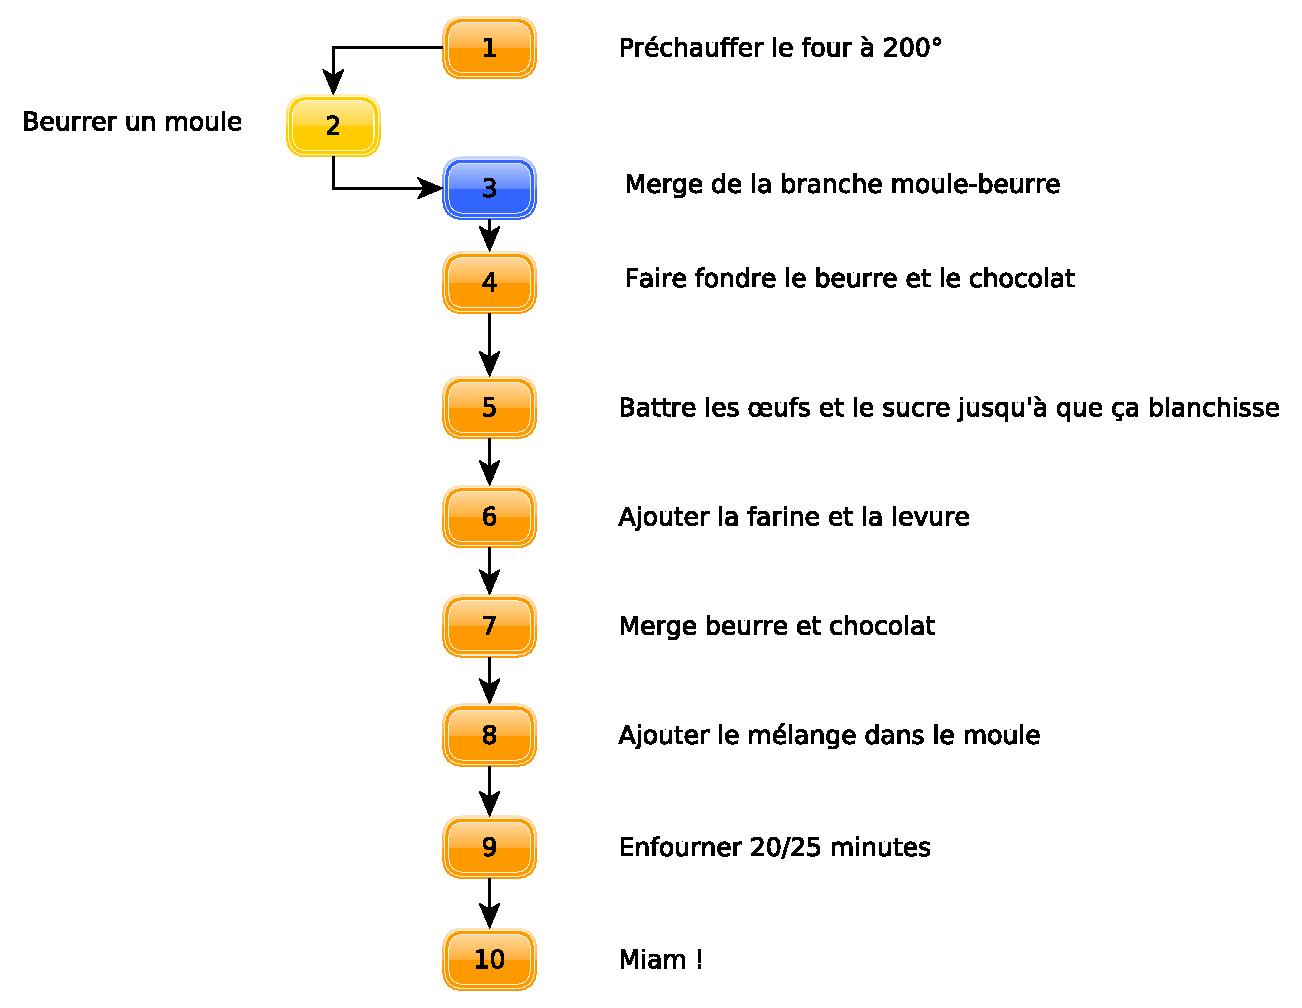
\includegraphics[width=6cm]{images/3-collaboration/ff.eps}
				\lstinputlisting[language=sh, linewidth=5cm]{merge-noff}%
			}
		\end{minipage}
		&
		\begin{minipage}{0.5\textwidth}
			\uncover<2->{
		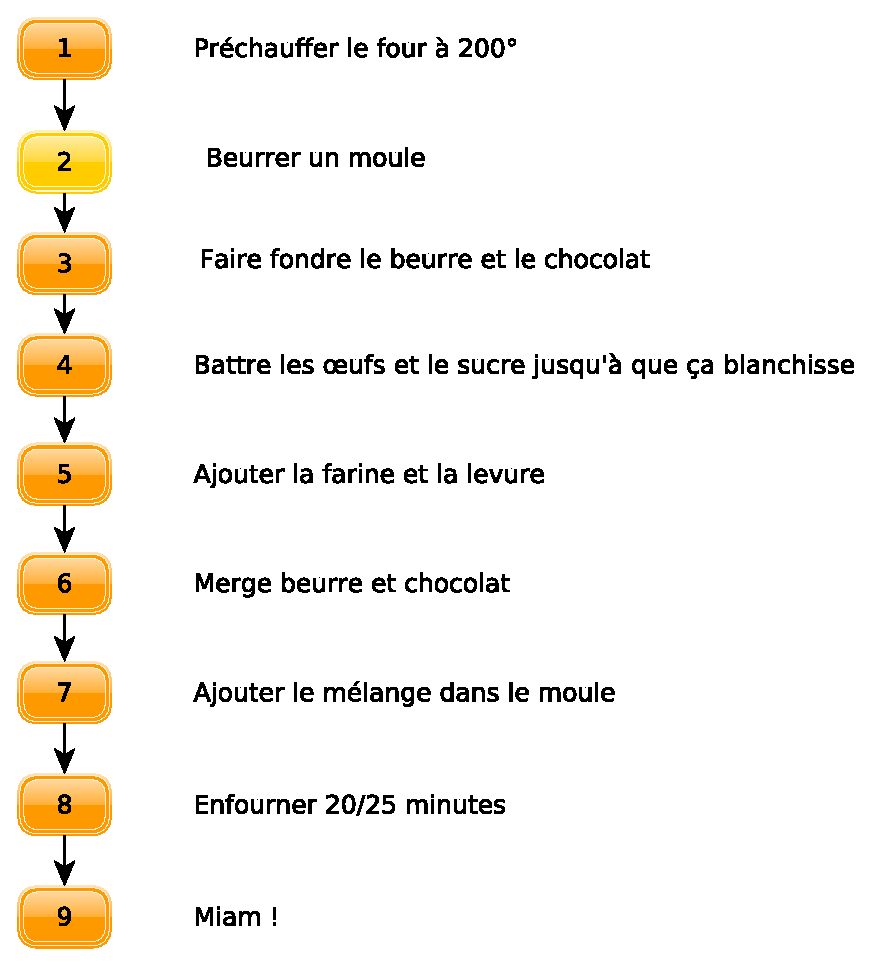
\includegraphics[height=5cm]{images/3-collaboration/ff2.eps}
	\lstinputlisting[language=sh,linewidth=5cm]{merge-moule}%
	}
		\end{minipage}
	\end{tabular}
\end{frame}

\begin{frame}{Le merge : le squash}
	\begin{tabular}{cc}
		\begin{minipage}{0.5\textwidth}
			\uncover<1->{
			\hspace{-1cm}
				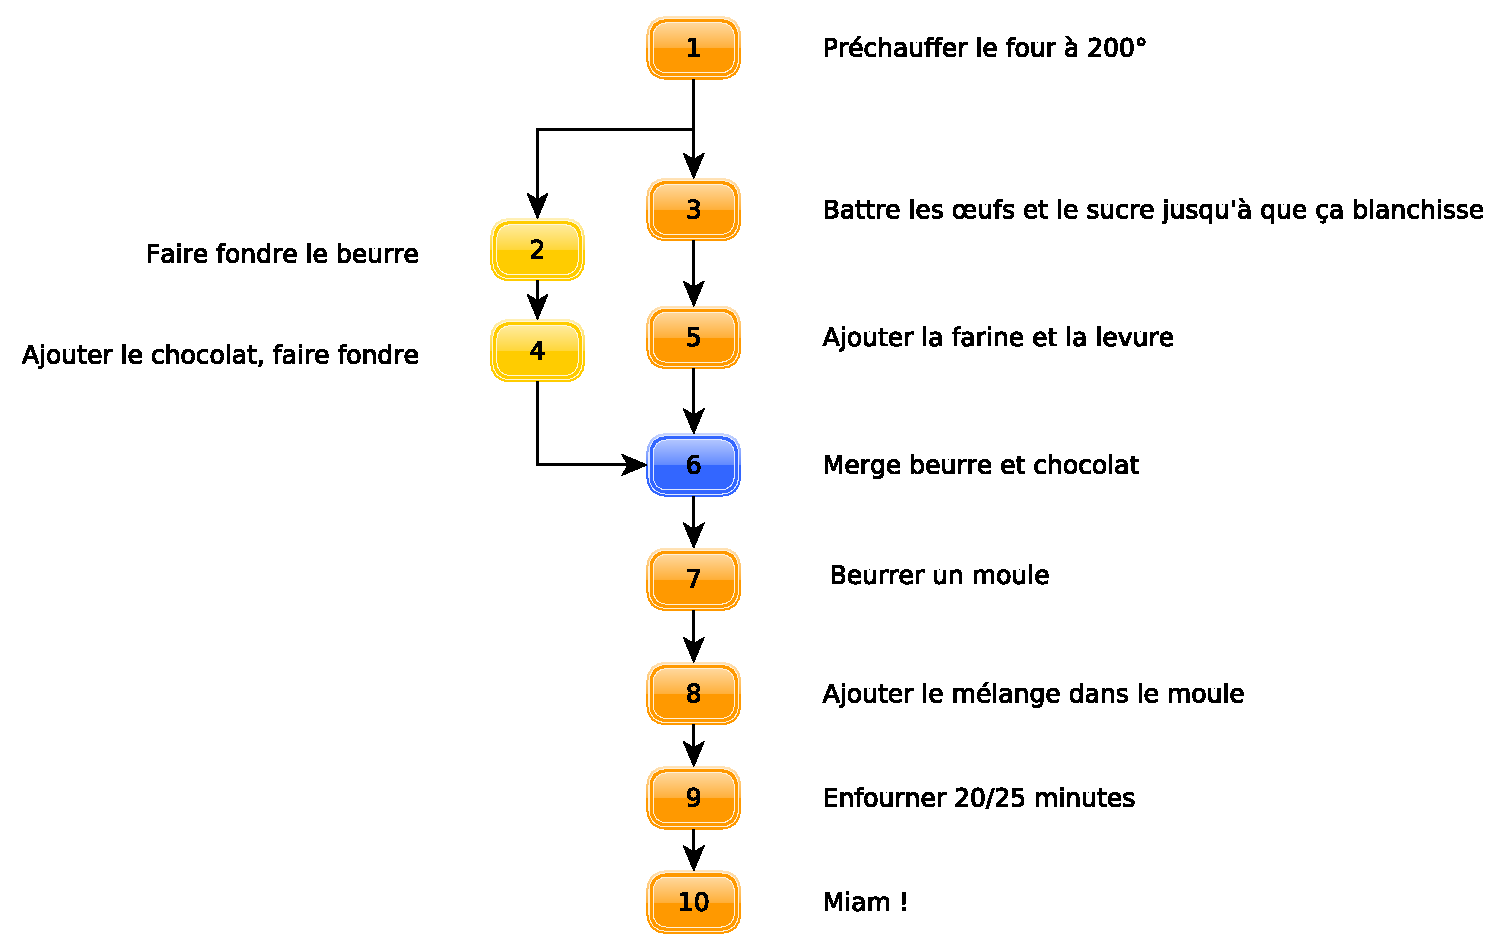
\includegraphics[width=7cm]{images/3-collaboration/merge.eps}
				\lstinputlisting[language=sh, linewidth=5cm]{merge}%
			}
		\end{minipage}
		&
		\begin{minipage}{0.5\textwidth}
			\uncover<2->{
		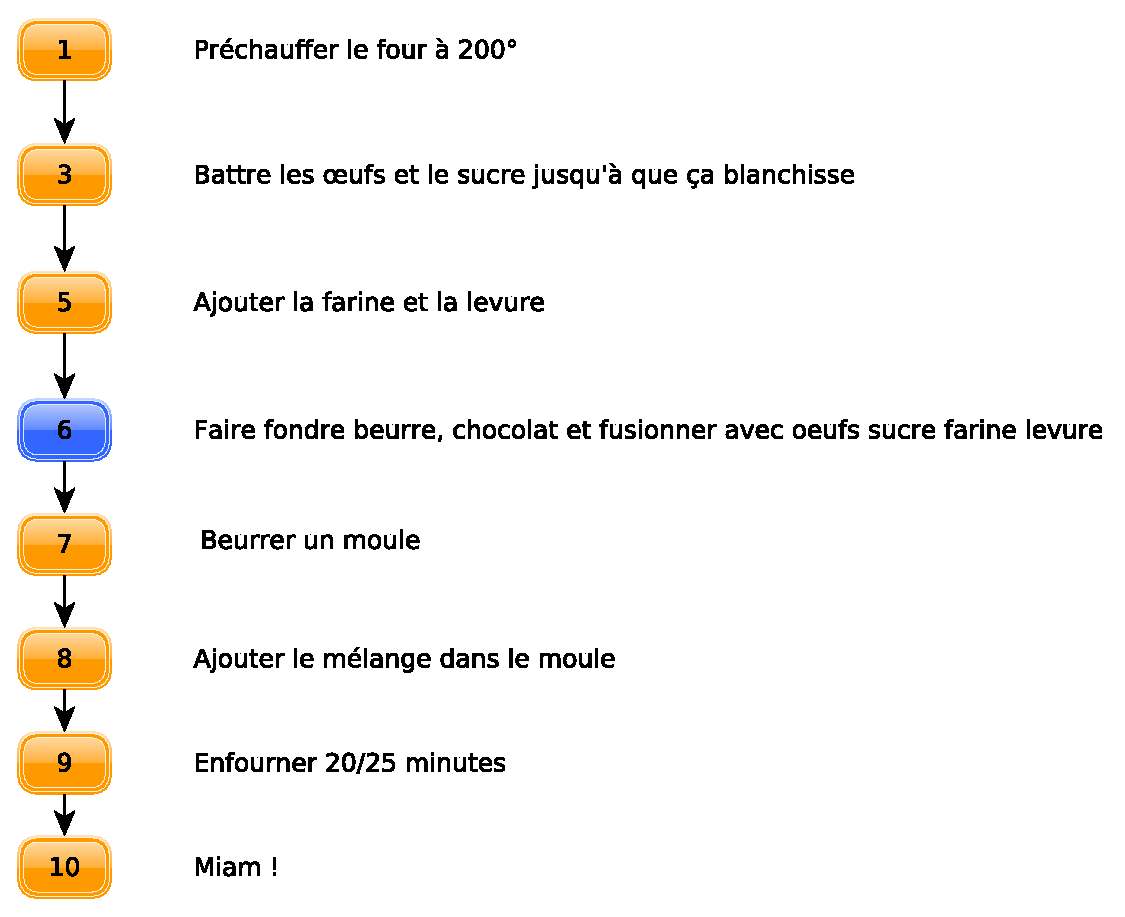
\includegraphics[height=4.5cm]{images/3-collaboration/mergesquash.eps}
	\lstinputlisting[language=sh,linewidth=5cm]{mergesquash}%
	}
		\end{minipage}
	\end{tabular}
\end{frame}

\begin{frame}{Le rebase : on veut un historique linéaire}
	\begin{tabular}{cc}
		\begin{minipage}{0.5\textwidth}
			\uncover<1->{
			\hspace{-1.5cm}
				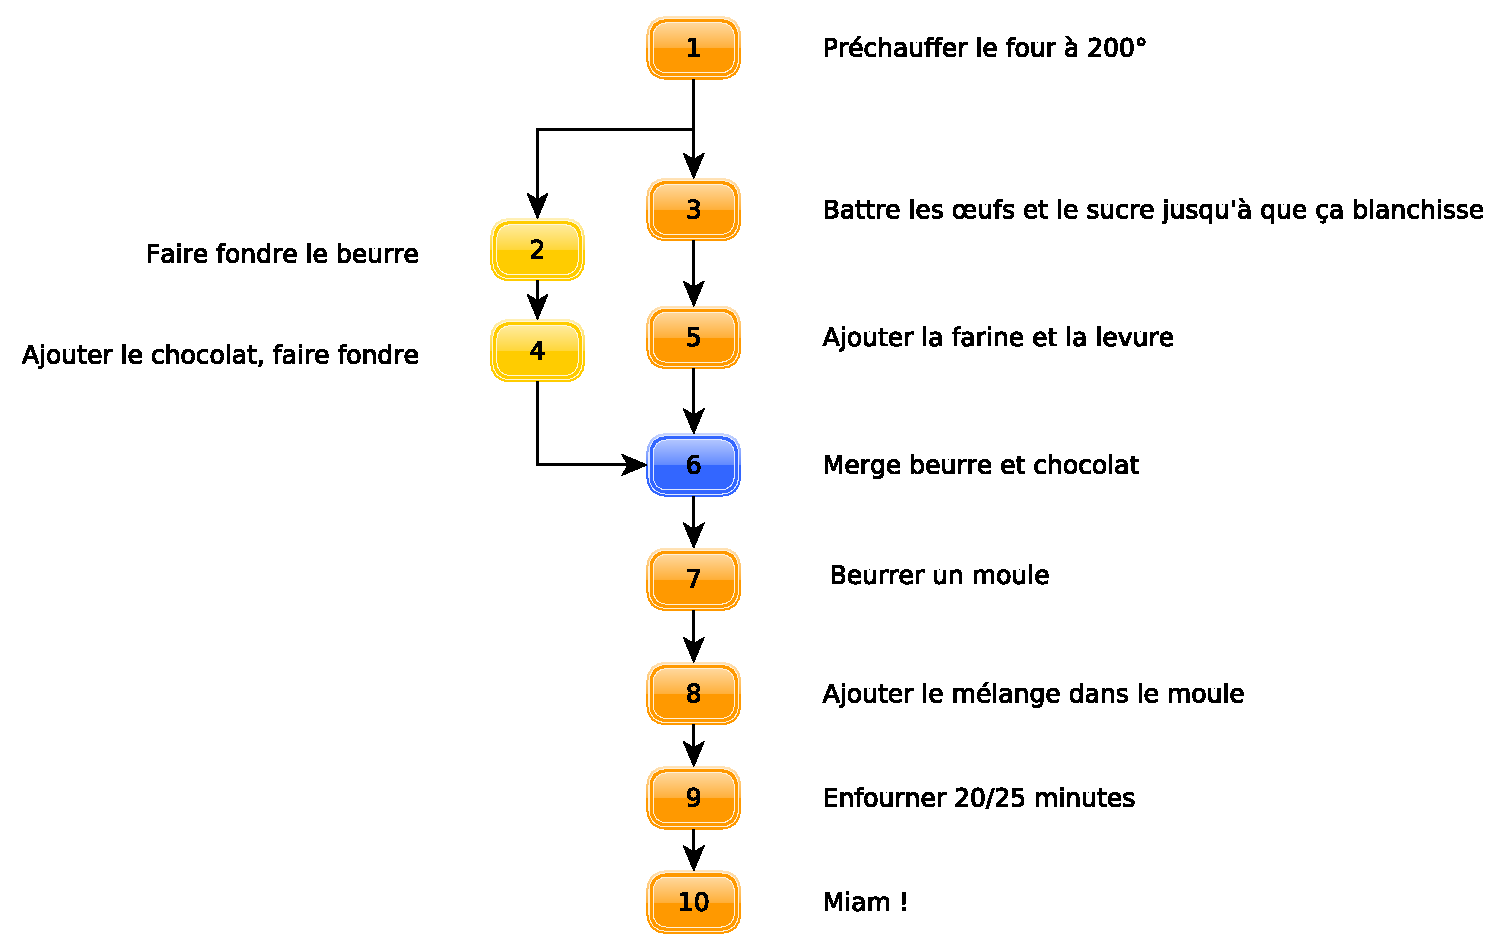
\includegraphics[width=7cm]{images/3-collaboration/merge.eps}
				\lstinputlisting[language=sh, linewidth=5cm]{merge}%
			}
		\end{minipage}
		&
		\begin{minipage}{0.5\textwidth}
			\uncover<2->{
			\hspace{-0.5cm}
		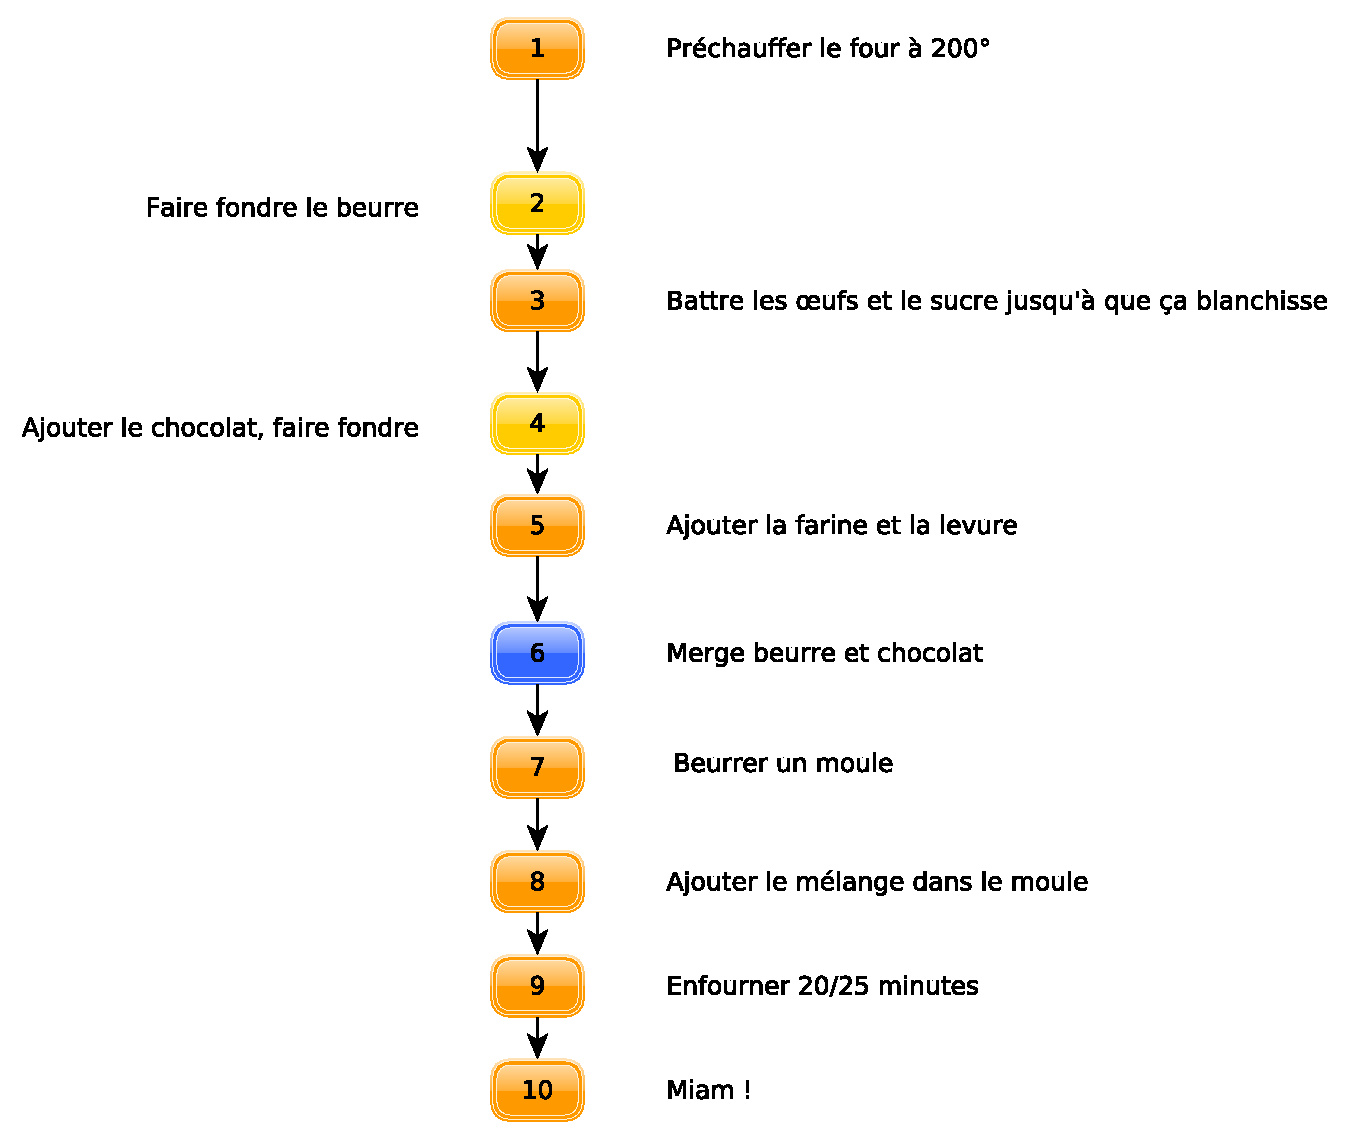
\includegraphics[height=5cm]{images/3-collaboration/rebase.eps}
	\lstinputlisting[language=sh,linewidth=5cm]{rebase}%
	}
		\end{minipage}
	\end{tabular}
\end{frame}
\begin{frame}{Le rebase : Attention à son utilisation}
	\begin{itemize}
		\item Jamais sur une branche partagée
			\begin{itemize}
				\item Un rebase réécrit l'historique et va donc changer les hash
			\end{itemize}
			\vfill
		\item Si la branche à été poussée
			\begin{itemize}
				\item Il faut faire un push force… Et donc écraser l'historique de la branche distante !
			\end{itemize}
			\vfill
		\item Principalement à utiliser pour : 
			\begin{itemize}
				\item Mettre à jour sa branche par rapport à la branche mère
				\item Réécrire son historique
			\end{itemize}
			\vfill
	\end{itemize}
\end{frame}


\begin{frame}{Le stash : mettre des modifications de côté}
	\begin{itemize}
		\item Utile pour pouvoir changer de brancher ou se mettre à jour sans commiter
		\item Gestion des conflits lors de l'application du stash 
	\end{itemize}
	\vfill
	\uncover<2->{
	\begin{itemize}
		\item Le stash est une pile : 
			\begin{itemize}
				\item \texttt{git stash} pour empiler 
				\item \texttt{git stash pop} pour dépiler
				\end{itemize}
		\item Possibilité d'y accéder comme une liste 
			\begin{itemize}
				\item \texttt{git stash list}
				\item \texttt{git stash apply stash\_name}
			\end{itemize}
	\end{itemize}
	}
\end{frame}

\begin{frame}{Le cherry-Pick}
\end{frame}

\section{Utilisation avancée}
\begin{frame}{Le {pull} devrait être interdit…}
	\uncover<1->{
	\begin{itemize}
		\item Par défaut, le pull peut être vu comme un alias : 
	\end{itemize}
	\lstinputlisting[language=sh, title=Un git pull si on est sur master]{pull}%
	}
	\begin{itemize}
		\item<2-> Si on est pas en fast-forward, le merge va créer une branche temporaire 
		\item<3-> Ne faire un pull que si on est en fast forward
		\item<4-> Sinon, il faut faire
	\end{itemize}
	\uncover<4->{
	\lstinputlisting[language=sh, title=Se mettre à jour si on est sur master]{fetch}%
	}
\end{frame}

\begin{frame}{Le rebase interactif : réécrire l'histoire}
	\begin{tabular}{cc}
		\begin{minipage}{0.5\textwidth}
	\begin{figure}[H]
		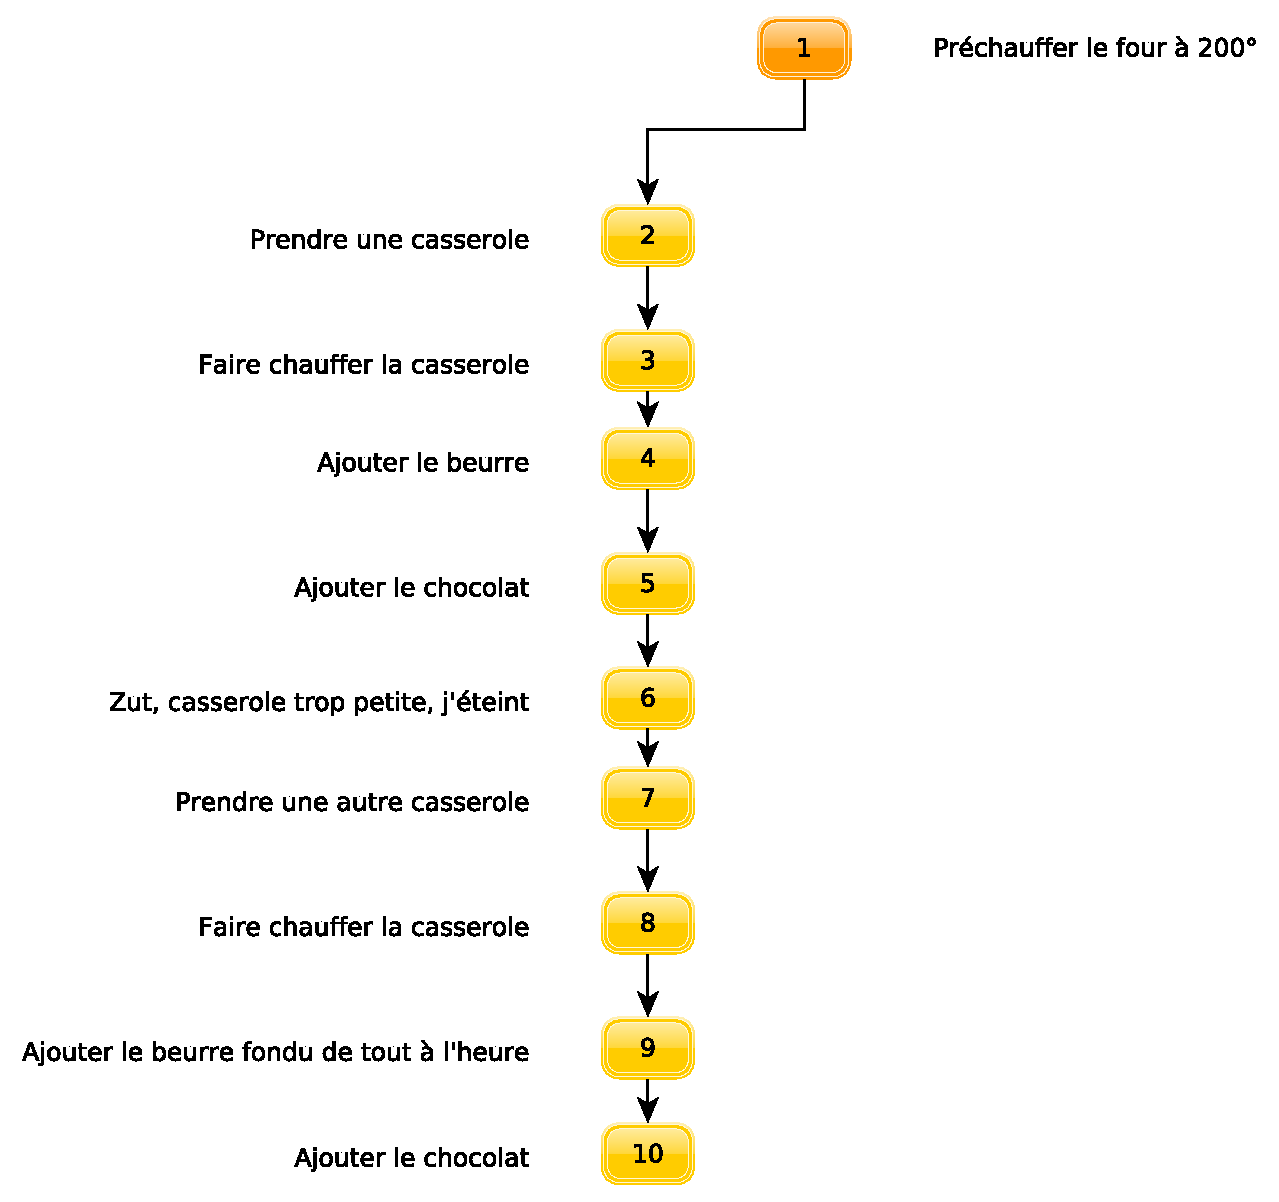
\includegraphics[height=6cm]{images/3-collaboration/rebaseinteractif.eps}
		\caption{Un historique pourri}
	\end{figure}
\end{minipage}
	&
	\begin{minipage}{0.5\textwidth}
		\pause
	\begin{figure}[H]
		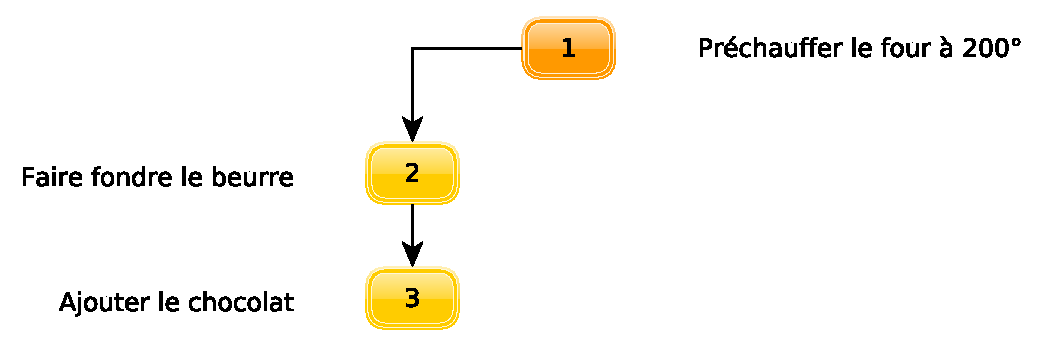
\includegraphics[width=5cm]{images/3-collaboration/rebaseinteractif_2.eps}
		\caption{Et après un peu de nettoyage}
	\end{figure}
\end{minipage}
	\end{tabular}
\end{frame}
\begin{frame}{Le rebase interactif : réécrire l'histoire}
	\lstinputlisting[language=sh, title=Utilisation du rebase interactif]{rebase-interactif}%
	\begin{itemize}
		\item<1-> \textbf{p, pick} : utiliser le commit (ne change rien)
		\item<2-> \textbf{r, reword} : utilise le commit, mais permet de changer le message
		\item<3-> \textbf{e, edit} : utilise le commit et s'arrête pour pouvoir changer le contenu du commit
		\item<4-> \textbf{s, squash} : fusionne avec le commit précédent
		\item<5-> \textbf{d, drop} : supprime le commit
	\end{itemize}
\end{frame}

\begin{frame}{Bisect : trouver d'où vient le bug}
	\uncover<1->{
	\begin{itemize}
		\item Savoir depuis quel commit l'application ne fonctionne plus 
	\end{itemize}
	\lstinputlisting[language=sh, title=Utilisation de git bisect]{bisect}%
	}
	\uncover<2>{
	\begin{itemize}
		\item Et si on a des tests automatisés ?
	\end{itemize}
	
	\lstinputlisting[language=sh, title=Utilisation de git bisect pour lancer les tests]{bisect2}%
	}

\end{frame}
\appendix
\section*{Conclusion}
\begin{frame}
\only<1,3>{
	\begin{figure}[H]
		\centering
		\vspace{-7px}
		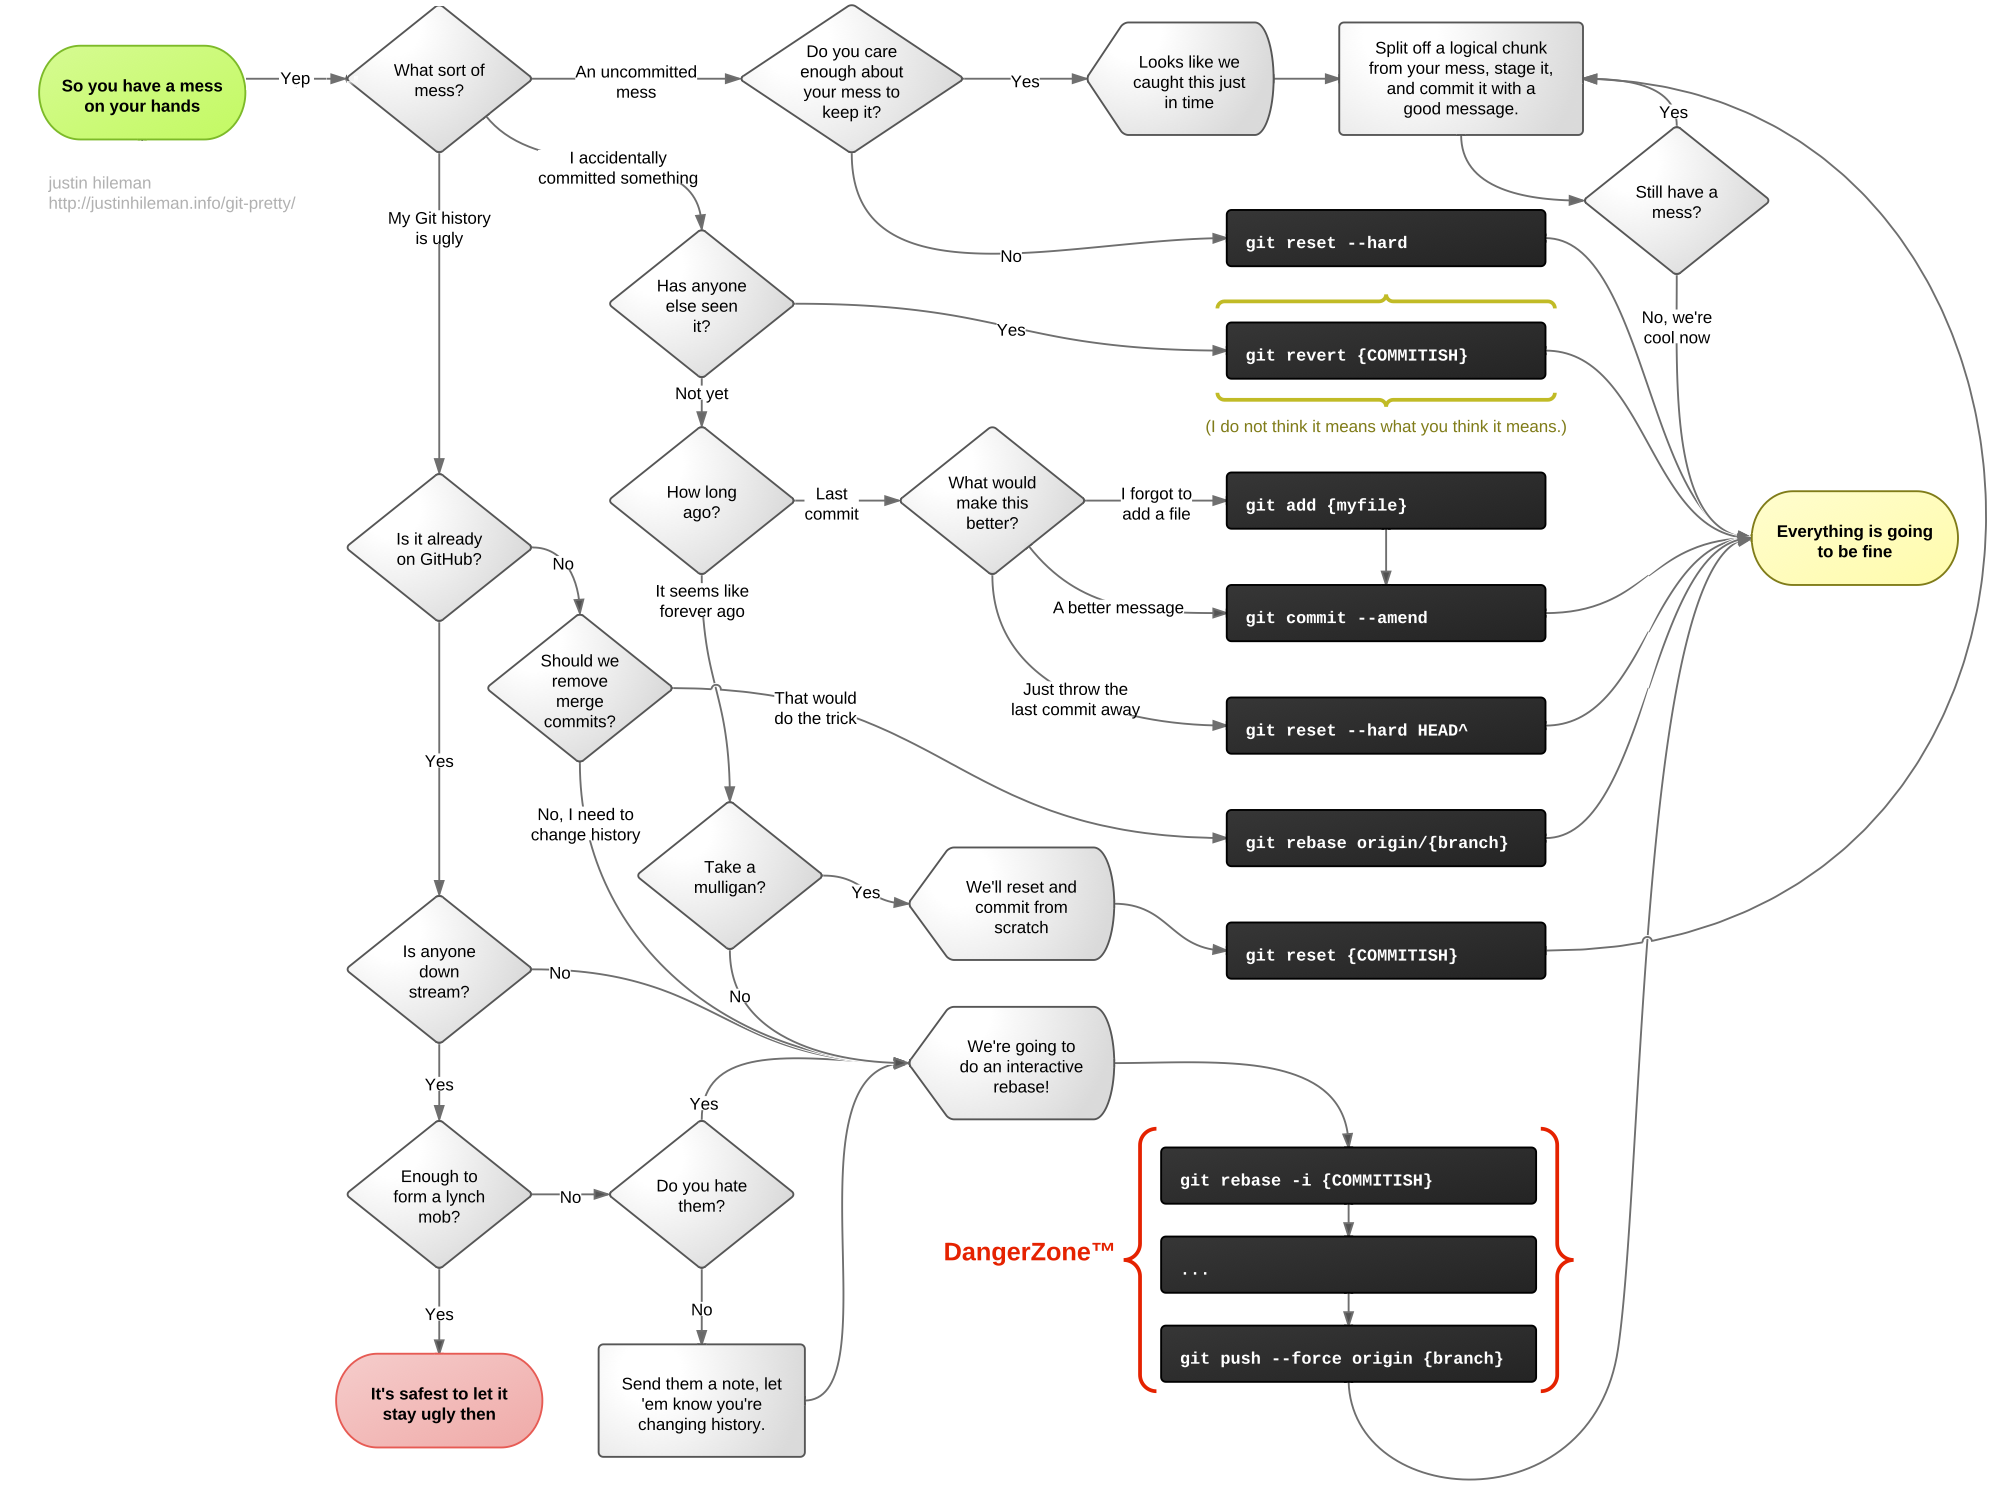
\includegraphics[width=9cm]{images/git-mess.png}
		\vspace{-10px}
		\caption{\textit{So, you have a mess on your hands ?}\footnote{\url{http://justinhileman.info/article/git-pretty/}}}
	\end{figure}
	}

	\only<2>{
	{
		\vspace{10.01cm}
		\hspace{0.5cm}
        \begin{tikzpicture}[remember picture,overlay]
            \node[at=(current page.center)] {
                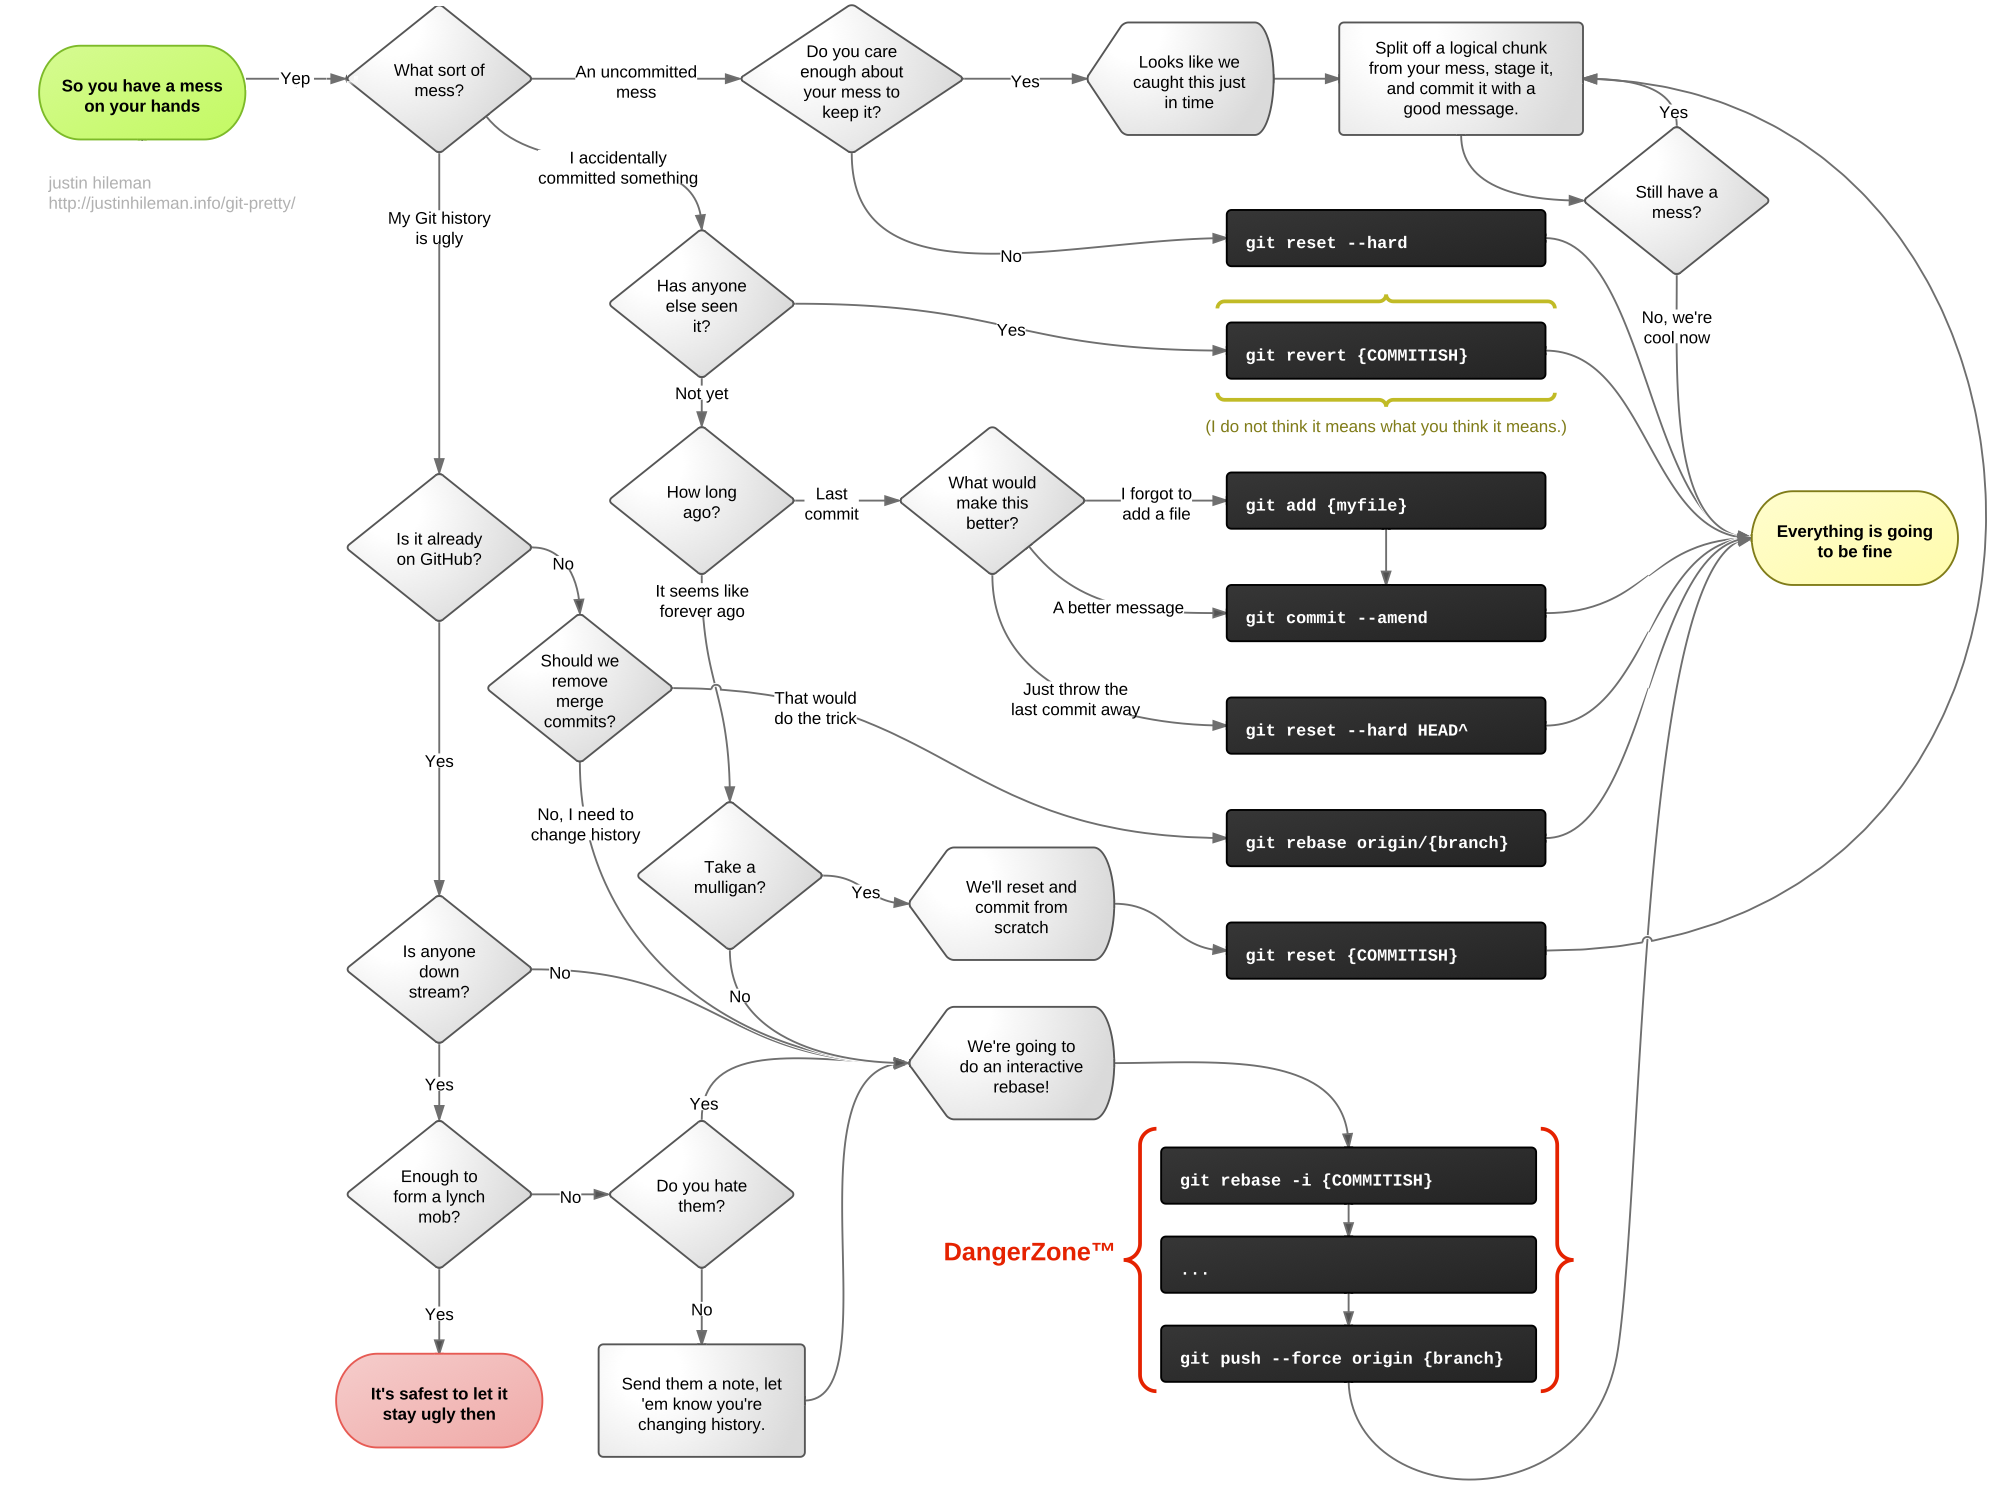
\includegraphics[keepaspectratio,
                                 height=1.05\paperheight]{images/git-mess.png}
            };
        \end{tikzpicture}
		}
		}
\end{frame}

\section*{Références}
\begin{frame}{Références}
		\centering
	\begin{tabular}{cc}
		
\includegraphics[height=4cm]{images/refs/oreally.jpg}&
		
\includegraphics[height=4cm]{images/refs/progit.png}\\
	\end{tabular}
	\vfill
	\begin{itemize}
		\item \footnotesize \texttt{\href{https://git-scm.com}{git-scm.com}}\\
			{Site officiel}
		\item \footnotesize \texttt{\href{https://learngitbranching.js.org}{learngitbranching.js.org}}\\
			{Apprendre Git de manière ludique}
		\item \footnotesize \texttt{\href{https://github.com/aroquemaurel/Presentation-beamer-Git}{github.com/aroquemaurel/Presentation-beamer-Git}}\\
			Les sources \LaTeX{} de cette présentation
	\end{itemize}
\end{frame}

\begin{frame}
\title{\centering Git, Essayons de reprendre le contrôle !}
\subtitle{}
\author{
	\centering
  Antoine de {\sc Roquemaurel}\\
	  \begin{tabular}{ccc}
		  
\includegraphics[height=7pt]{images/twitter.png}~satenske
	  \end{tabular}
	  \\
  {\footnotesize
	  \vspace{10px}
		Développeur Java consultant chez Tech Advantage\\
  }
}
\date{
	{
	  \begin{tabular}{ccc}
		  
\includegraphics[height=1.cm]{images/logo_extia}\hspace{20px} & 
		  
\includegraphics[height=1.cm]{images/meetup_by_extia} & 
		  \hspace{10px} 
\includegraphics[height=1cm]{images/logo_git}
	  \end{tabular}
	}
	\\
	\vspace{10px}
	Meetup Java / C\# du 28 Mars 2019\\\vspace{0.9cm}
	\vfill
	\includegraphics[width=1cm]{images/cc-by.eps} 
	\begin{minipage}{0.8\textwidth} 
		\tiny Cette œuvre est mise à disposition selon les termes de la Licence Creative Commons By 4.0\\
	\end{minipage}
}
\titlepage
\end{frame}

\end{document}
